% ICRA 2027 contributed paper -- Overleaf / camera-ready source of truth
% Upload this folder (or the zip) to Overleaf: New Project → Upload Project
\documentclass[conference]{IEEEtran}
\IEEEoverridecommandlockouts

\usepackage{graphicx}
\usepackage{amsmath,amssymb}
\usepackage{booktabs}
\usepackage{hyperref}
\usepackage{cite}
\usepackage{xcolor}
\usepackage{url}

\graphicspath{{figures/}}

\title{Preserving Strategy Specialization under Progressive Parameter Sharing\\
in Multi-Robot Policies}

\author{
  \IEEEauthorblockN{Anonymous Authors}
  \IEEEauthorblockA{Anonymous Institution\\
  \texttt{anonymous@example.com}}
}

\begin{document}
\maketitle

% Reading/writing order for polish (experimental framing FROZEN):
% Problem Setup → Methodology → Results → Discussion → Conclusion
% → Related Work / Abstract final polish.
% Related Work sits after Introduction in the compiled PDF (standard ICRA layout).

\section*{Abstract}
%======================================================================

Multi-robot teams operating against heterogeneous adversaries may require
qualitatively different coordination strategies under different opponent
regimes. Deploying a separate network for every regime preserves specialization
but scales poorly; a single shared policy conditioned on a discrete strategy
code is more compact, yet strategically important behavior can be difficult to
preserve under parameter sharing. We study this question in a partially
observable maritime multi-robot Capture-the-Flag task with two scripted opponent
regimes. We train independent opponent-specific PPO experts with complementary
closed-loop specialization, distill their matched-state behaviors into discrete
modes of a strategy-conditioned controller $\pi_\theta(a\mid o,z)$, and
progressively increase shared policy structure while measuring whether
payoff-level specialization survives. Evaluation separates action imitation,
action-distribution separation, and closed-loop payoff specialization. On a
matched $128$-seed protocol, sharing only the perception encoder preserves
specialization
($\Delta_A=+0.266\,[+0.148,+0.383]$, $\Delta_B=+0.164\,[+0.047,+0.281]$)
with no detectable paired loss relative to a zero-sharing expert dispatch
control; sharing the policy backbone still clears the absolute criterion but
yields detectable specialization loss despite comparable imitation fidelity; and
sharing macro-action outputs no longer satisfies the specialization criterion
($\mathrm{LCB}_{95}(\Delta_A)=0$). PPO is used only as the expert-learning
engine; the primary experimental variable is progressive parameter sharing after
matched-state distillation.

\section{Introduction}
%======================================================================

Multi-robot systems that operate against heterogeneous environments or
adversaries often cannot rely on a single coordination style. Different opponent
behaviors can require qualitatively different team strategies---for example, a
broad zone defense may favor one form of team organization, while a compact,
reactive defense favors another. Learning policies that express the right
strategy for the encountered regime is therefore a central robotics problem,
not merely a representation-learning detail.

Storing a separate neural policy for every operating regime preserves
specialization but does not scale well as the number of regimes grows. Memory,
deployment complexity, and maintenance cost all increase with the number of
independent networks. A natural alternative is one shared multi-robot policy
conditioned on a small discrete \emph{strategy code}: the code selects which
opponent-conditioned behavior the shared policy should express.

Parameter sharing, however, can erase strategically important differences even
when average action imitation remains high. Closed-loop coordination depends on
temporally extended decisions; agreement on individual actions does not
automatically imply that each conditioned mode retains its intended task
advantage. The scientific question of this paper is therefore:

\begin{quote}
\emph{Can a single strategy-conditioned multi-robot policy preserve multiple
opponent-specific strategies, and how much neural-network parameter sharing can
be introduced before those strategies interfere with one another?}
\end{quote}

Existing latent-policy and multi-agent reinforcement learning methods have shown
that a shared policy can represent diverse behaviors, roles, or
opponent-conditioned responses. However, substantially less attention has been
paid to whether strategically distinct behaviors remain preserved as
increasingly large portions of the policy are forced to share parameters. This
distinction is important because high action-level imitation fidelity does not
necessarily imply preservation of closed-loop strategic behavior.

We therefore study strategy preservation under progressive policy sharing in a
multi-robot adversarial task. The pipeline is intentionally staged so that each
box has a distinct role:
\begin{quote}
\emph{PPO learns the experts;}
\emph{matched-state distillation creates discrete shared strategy modes;}
\emph{progressive parameter sharing is the primary experimental variable;}
\emph{closed-loop crossover is the validation.}
\end{quote}
Concretely, we train two independent opponent-specific PPO specialists
($\pi_A$ vs.\ Regime~A / OP6; $\pi_B$ vs.\ Regime~B / OP7), validate their
complementary payoff specialization, and construct a zero-sharing structural
control that dispatches the verbatim experts by strategy code (Share-0). We then
distill the experts into modes $z_0\!\sim\!\pi_A$ and $z_1\!\sim\!\pi_B$ of
shared controllers under a \emph{common} distillation recipe while progressively
tying modules (Share-Encoder $\rightarrow$ Share-Backbone $\rightarrow$
Share-Macro), asking where closed-loop specialization survives or collapses.
Among the distilled rungs, the primary experimental variable is the location and
amount of parameter sharing; Share-0 is the bit-exact expert dispatch reference
against which paired losses are measured. We do \emph{not} present this core as
a new PPO algorithm.

The main contributions of this work are:
\begin{enumerate}
  \item A strategy-conditioned expert-distillation framework that grounds
  discrete modes $z$ in independently learned, crossover-validated PPO experts
  via matched-state supervision, isolating strategy differences from
  state-distribution differences.
  \item A progressive parameter-sharing study that isolates the effect of
  sharing perception, policy-backbone, and action-output modules on
  opponent-conditioned specialization while holding the distillation recipe,
  data, schedule, seeds, and payoff criterion fixed among distilled rungs---with
  a bit-exact expert-dispatch Share-0 control as the zero-sharing reference.
  \item A measurement hierarchy that refuses to equate imitation or
  action-distribution separation with closed-loop strategic meaning: a
  $z_0$/$z_1$ pair counts only if changing $z$ changes payoff preference
  against the opponent regimes.
\end{enumerate}

%======================================================================

\section{Related Work}
\label{sec:related}
%======================================================================

Latent-conditioned multi-agent RL, emergent-role methods (e.g., ROMA), latent
exploration (e.g., MAVEN), and partner/opponent latent models (e.g., LILI)
study how discrete or continuous latent variables can induce behavioral
diversity or coordination. Multi-agent and policy distillation transfer
expertise into compact or shared controllers, and parameter sharing is a
standard MARL efficiency tool. Our question is different: \emph{after}
establishing independently learned, payoff-specialized strategies, how does
\emph{progressively increasing architectural sharing} affect their closed-loop
specialization under a fixed distillation recipe and matched-seed payoff gate?
We also situate the task relative to multi-robot CTF platforms such as
Aquaticus / Pyquaticus, which provide the maritime adversarial setting but do
not address this sharing-preservation measurement.

%======================================================================

\section{Problem Setup}
\label{sec:setup}
%======================================================================

\subsection{Environment and agents}

We study a partially observable, adversarial multi-robot setting instantiated
as a nominal $2$-vs-$2$ naval Capture-the-Flag task on a symmetric maritime
arena. Blue is the learned multi-robot team; Red is a scripted or frozen
adversarial opponent. Each side controls $|B|=|R|=2$ autonomous surface vessels.
We model the interaction as a finite-horizon partially observable Markov game
\[
G =
\left(
\mathcal{N},\mathcal{S},\{\mathcal{A}_i\}_{i\in\mathcal{N}},P,
\{r_i\}_{i\in\mathcal{N}},\{\Omega_i\}_{i\in\mathcal{N}},\{O_i\}_{i\in\mathcal{N}},\gamma
\right),
\]
with $\mathcal{N}=B\cup R$.

At each simulator tick $t$, agent $i$ receives a local observation
$o_{i,t}\sim O_i(\cdot\mid s_t)$ and may request a temporally extended
\emph{macro-action} together with a target. The macro vocabulary is
$\{\texttt{GO\_TO},\texttt{GRAB\_MINE},\texttt{GET\_FLAG},\texttt{PLACE\_MINE},\texttt{GO\_HOME}\}$.
For reproducibility, the joint action is represented as
$\mathrm{MultiDiscrete}([5,50,5,50])$ (per agent: a $5$-way macro and a
$50$-way target). The joint action induces $s_{t+1}\sim P(\cdot\mid s_t,a_t)$.

Each team's flag is anchored at its home base; a carrier that returns the enemy
flag alive scores a capture. Mines are stationary hazards that create
area-denial and ambush dynamics.

\subsection{Asynchronous macro-action decision points}

An accepted macro-action is held for a macro-specific number of ticks before the
agent may choose a new one
($\texttt{GO\_TO}=4$, $\texttt{GRAB\_MINE}=3$, $\texttt{GET\_FLAG}=4$,
$\texttt{PLACE\_MINE}=2$, $\texttt{GO\_HOME}=4$). Agent $i$ carries a countdown
$c_{i,t}$; a newly requested macro is accepted only when
\[
d_t^i=\mathbb{I}\!\left[c_{i,t}\le 0\right].
\]
When $d_t^i=0$, the legal-action mask collapses to the already-committed macro,
so the network output is not an executable decision. Because hold lengths differ
by macro and agents commit independently, decision boundaries are asynchronous.
For policy evaluation and supervision, the task is therefore better viewed as a
semi-Markov decision process over commitment decisions than as a flat per-tick
Markov decision process.

\subsection{Opponent regimes}

Red is drawn from one of two scripted defensive philosophies that we call
\emph{opponent regimes}:
\begin{itemize}
  \item \textbf{Opponent Regime~A:} broad / passive zone defense.
  \item \textbf{Opponent Regime~B:} compact / reactive defense.
\end{itemize}
The two regimes are designed to elicit contrasting strategic responses from
Blue rather than represent two difficulty levels of the same opponent behavior.
Implementation identifiers used for reproducibility (configuration overlay
\textbf{OP6} for Regime~A; canonical \textbf{OP7} for Regime~B), together with
frozen behavior-tree parameters such as
$\texttt{defender\_zone\_frac}$ and $\texttt{threat\_radius}$, are recorded in
the experiment configuration and are not repeated as conceptual labels in the
main narrative.

We do not assume a priori that the two regimes require different Blue
strategies. An \emph{opponent-conditioned strategy-preference test} measures
whether a GUARD-biased response is preferred over a BREACH-biased response under
Regime~A, and the reverse contrast under Regime~B, with pass condition
$\mathrm{LCB}_{95}>0$ on each contrast. This empirical test establishes whether
the regimes induce complementary strategic demand. If one Blue policy were
simply better against both regimes, a single shared behavior would be
appropriate rather than a specialization problem.

\subsection{Strategy-conditioned policies}

Let $\pi_\theta(a\mid o,z)$ denote a shared multi-robot policy conditioned on a
discrete \emph{strategy code} $z\in\{z_0,z_1\}$. The strategy code selects which
opponent-conditioned behavior the shared policy should express. The intended
deployment mapping is $z_0\mapsto\text{Regime~A}$ and $z_1\mapsto\text{Regime~B}$;
once fixed, this assignment is never flipped. Let $V(z,p)$ denote the win rate
when deploying with strategy code $z$ against opponent regime
$p\in\{A,B\}$, estimated over a held-out seed block.

Independently trained \emph{strategy-specific expert policies} $\pi_A$ and
$\pi_B$ are the source behaviors: each is trained against one regime with no
shared parameters and no strategy-code mechanism. Their bit-exact $z$-dispatch
wrapper is Share-0 (Section~\ref{sec:sharing}). A single \emph{generalist}
policy $\pi_G$ trained on the mixed opponent distribution without a strategy
code provides a single-policy baseline.

\subsection{Strategy-specialization criterion}
\label{sec:specialization}

We require more than behavioral diversity. For two strategy codes to represent
meaningful specialization, each code must provide higher task success than the
alternative code in its intended opponent regime. A policy is considered
strategy-specialized only if each strategy code significantly outperforms the
alternative code in the opponent regime for which it is intended.

Formally, define
\[
\Delta_A = V(z_0,A)-V(z_1,A),
\qquad
\Delta_B = V(z_1,B)-V(z_0,B).
\]
The \emph{strategy-specialization criterion} (equivalently, the two-sided
\emph{specialization crossover} pattern) requires
\[
\mathrm{LCB}_{95}(\Delta_A)>0
\quad\wedge\quad
\mathrm{LCB}_{95}(\Delta_B)>0,
\]
evaluated by a paired percentile bootstrap over the held-out seeds with
$n_{\mathrm{boot}}=20{,}000$, $\alpha=0.05$, and the seed as the resampling
unit. The binary win indicator is the primary outcome because it is the
deployment quantity used by every specialization evaluation.

Independent-expert specialization is reported on a held-out $64$-seed block.
All parameter-sharing comparisons use the matched $128$-seed paired protocol of
Section~\ref{sec:matched}.

\subsection{Scope of claims}

Primary claims apply to the nominal $2$-vs-$2$ environment, the two opponent
regimes above, the specific training recipe, and the fixed evaluation
implementation. Scaling to $4$-vs-$4$ and $6$-vs-$6$, and robustness
perturbations such as localization noise, motion uncertainty, and control delay,
are external-validity experiments. Until completed, they are not used as evidence
for the primary sharing conclusions and are not used to select the primary
architecture.

%======================================================================

\section{Methodology}
\label{sec:method}
%======================================================================

\paragraph{Overview.}
The successful method is not a new PPO variant. It is
\emph{opponent-specific PPO expert training}, followed by
\emph{matched-state strategy-conditioned distillation}, followed by
\emph{progressive parameter sharing} with a closed-loop payoff gate.

\begin{figure}[t]
\centering
\fbox{\parbox{0.96\linewidth}{\small
\textbf{Algorithm 1}~~Strategy-conditioned expert distillation and progressive sharing\\[0.4em]
\textbf{Require:} regimes $A,B$; seeds; KL distill budget; bootstrap gate\\
1:\quad Train independent PPO experts $\pi_A$ (vs~$A$), $\pi_B$ (vs~$B$)\\
2:\quad Verify specialist crossover: $\Delta_A>0$, $\Delta_B>0$ with LCB$_{95}>0$\\
3:\quad Build Share-0: bit-exact $z$-dispatch of verbatim experts (structural control)\\
4:\quad Collect a shared state set $\{s\}$ (both experts queried on each $s$)\\
5:\quad For share $\in\{$Encoder, Backbone, Macro$\}$: distill under a \emph{common} recipe\\
\quad\quad with the corresponding modules tied; freeze the terminal checkpoint\\
6:\quad Evaluate each distilled rung on matched seeds: absolute $\Delta$ gate + paired $D$ vs Share-0\\
7:\quad Report where specialization is preserved, degraded, or lost\\
\textbf{Fixed among distilled rungs:} data, schedule, seeds, CUDA path, no post-hoc ckpt selection.\\
\textbf{Note:} Share-0 is constructed, not distilled; Enc$\rightarrow$Back$\rightarrow$Macro varies sharing only.
}}
\caption{Reproducible Claim-A pipeline. PPO is the expert engine; among distilled rungs the primary experimental variable is progressive parameter sharing; closed-loop $\Delta$/$D$ is the validation.}
\label{alg:pipeline}
\end{figure}

\subsection{Opponent-specific PPO experts}

\textbf{Independent specialists.}
We train strategy-specific experts $\pi_A$ and $\pi_B$ with a standard
opponent-specific multi-agent PPO recipe under matched conditions---one policy
against Regime~A / OP6, one against Regime~B / OP7---with no shared parameters
and no strategy-code mechanism. PPO's role here is only to produce behavioral
experts with demonstrated complementary payoff specialization; it is not the
claimed algorithmic novelty. These experts are the teachers for distillation and
the verbatim actors behind Share-0.

\textbf{Generalist baseline.}
We also evaluate $\pi_G$, a single policy trained on the mixed opponent
distribution with no strategy-code mechanism. The generalist provides a
single-policy baseline trained on the mixed opponent distribution.

\subsection{Matched-state strategy-conditioned distillation}
\label{sec:distill}

Treating $\pi_A$ and $\pi_B$ as behavioral experts rather than as the final
shared controller, we transfer their behaviors into one strategy-conditioned
policy $\pi_\theta(a\mid o,z)$ by supervised distillation, with
$z_0$ meaning ``behave like the A expert'' and $z_1$ meaning ``behave like the
B expert.'' Both experts are queried on the \emph{same} stored states, so
differences between conditioned outputs are attributable to expert strategies
rather than different state visitation distributions
($s\!\sim\!d_{\pi_A}$ vs.\ $s\!\sim\!d_{\pi_B}$).

The distillation objective is
\[
\mathcal{L}_{\mathrm{distill}}
=
\tfrac{1}{2}D_{\mathrm{KL}}\!\left(\pi_A(\cdot\mid s)\,\|\,\pi_\theta(\cdot\mid s,z_0)\right)
+
\tfrac{1}{2}D_{\mathrm{KL}}\!\left(\pi_B(\cdot\mid s)\,\|\,\pi_\theta(\cdot\mid s,z_1)\right),
\]
evaluated per action head over masked distributions and averaged over
decision-eligible heads only ($d_t^i=1$). Only actor parameters are optimized;
critic parameters remain unchanged and are verified immobile. Training runs a
fixed number of epochs with no early stopping and no checkpoint selection; the
terminal checkpoint is the sole artifact.

We maintain three measurement levels and do not conflate them:
\begin{itemize}
  \item \textbf{Action-level imitation:} argmax agreement and KL divergence
  relative to the matched expert.
  \item \textbf{Strategy separation:} Jensen--Shannon divergence between the
  two conditioned action distributions.
  \item \textbf{Closed-loop strategy specialization:} $V(z,p)$, $\Delta_A$,
  $\Delta_B$, and the paired-bootstrap criterion of
  Section~\ref{sec:specialization}.
\end{itemize}
High action-level imitation does not logically imply task-level specialization.
Different strategy-conditioned action distributions likewise do not logically
imply payoff-relevant specialization. The payoff-based criterion is the primary
task-level definition.

\subsection{Attempted strategy-preserving fine-tuning (negative result)}
\label{sec:spppo}

We separately evaluated Counterfactual Strategy Correction (CSC) and
Strategy-Preserving Fine-Tuning (SPFT) as interventions for preserving
specialization during continued PPO optimization (SP-PPO~$=$~PPO+CSC+SPFT).
Neither recovered the prespecified closed-loop specialization criterion under
frozen matched protocols. Because these interventions are \emph{not} responsible
for the successful progressive-sharing results, we report their complete
formulation and sealed evaluation in the supplementary material rather than the
main text.

\subsection{Progressive parameter sharing (primary experimental variable)}
\label{sec:sharing}

Having established payoff-specialized experts and a bit-exact Share-0 dispatch
control, we ask: how much neural representation can two strategically distinct
behaviors share before closed-loop specialization disappears? For
Share-Encoder, Share-Backbone, and Share-Macro we hold the distillation recipe,
dataset, schedule, and evaluation seeds fixed and vary only which modules are
tied between the two strategy branches. Sharing is cumulative. Among these
distilled rungs, the primary experimental variable is the location and amount of
parameter sharing.

Share-0 is \emph{not} produced by that distillation: it is a structural
zero-sharing control that installs the frozen experts behind a $z$-dispatch
wrapper (bit-exact logit match). Paired contrasts $D$ vs.\ Share-0 therefore
ask whether a distilled shared controller matches the structural control's
specialization; they do not claim that Share-0$\rightarrow$Share-Encoder
changes only a sharing flag. The clean single-axis comparison is
Share-Encoder$\rightarrow$Share-Backbone$\rightarrow$Share-Macro.

\begin{table}[t]
\centering
\caption{Progressive parameter-sharing conditions. Share-0 is a bit-exact
expert-dispatch control (not distilled). Share-Encoder/Backbone/Macro share a
common distillation recipe; only tied modules change among those three.}
\label{tab:sharing}
\begin{tabular}{lll}
\toprule
\textbf{Condition} & \textbf{Shared components} & \textbf{Strategy-specific components} \\
\midrule
Share-0: Independent Experts
  & None
  & Entire actor \\
Share-Encoder: Shared Perception
  & Perception encoder
  & Backbone + outputs \\
Share-Backbone: Shared Perception + Backbone
  & Encoder + MLP backbone
  & Strategy branches + outputs \\
Share-Macro: Shared Backbone + Macro-Action Output
  & Encoder + backbone + macro-action outputs
  & Target-selection outputs \\
\bottomrule
\end{tabular}
\end{table}

Each condition uses complete actors of the experts' own architecture class,
thereby reducing the likelihood that performance differences are explained solely
by reduced per-strategy capacity. Module tying is verified by object identity
and unique-parameter arithmetic. A mixed-$z$ minibatch gives each shared module
gradient from both strategies in the same step.

\paragraph{Share-0 (structural control).}
Share-0 installs $\pi_A$ and $\pi_B$ behind a strategy-code dispatch wrapper with
zero shared parameters, verified bit-exact against both experts on the
evaluation device. It establishes that the dispatch-and-evaluate path can
express specialization when no parameters are shared and when no distillation
has occurred.

\subsection{Matched-seed paired evaluation}
\label{sec:matched}

All parameter-sharing conditions are evaluated on the same $128$ held-out
episode seeds as the Share-0 reference. For each seed, we compute the change in
specialization contrast relative to Share-0, yielding a paired estimate that
controls for variation in episode difficulty. The Share-0 outcomes on this
matched set are fixed before evaluating subsequent sharing conditions.

The primary statistics are
\[
D_A=\mathbb{E}_s\!\left[\Delta_A^{\mathrm{(cond)}}(s)-\Delta_A^{\mathrm{(Share\textrm{-}0)}}(s)\right],
\qquad
D_B=\mathbb{E}_s\!\left[\Delta_B^{\mathrm{(cond)}}(s)-\Delta_B^{\mathrm{(Share\textrm{-}0)}}(s)\right],
\]
under a paired bootstrap. We declare a detectable sharing-associated reduction
in specialization on a regime only if $\mathrm{UCB}_{95}(D_p)<0$: that is, the
upper $95\%$ confidence bound on the paired change lies below zero.

Because CPU and CUDA execution can produce different closed-loop trajectories
despite identical nominal seeds, all primary paired comparisons use a fixed CUDA
execution path. Diagnostics collected on CPU are scoped to the CPU-generated
state distribution.

\subsection{Imitation-fidelity control}
\label{sec:fidelity}

To interpret a reduction in specialization as associated with representation
sharing, compared models must reproduce their expert policies with similar
fidelity. We therefore define an imitation-fidelity comparability band:
final holdout argmax agreement must lie within $0.010$ of the Share-Encoder
reference agreements on the same holdout set. This band is an
\emph{interpretation criterion}, not a success gate and not a theoretically
privileged threshold. Continuous agreement and KL values are reported for every
condition regardless of band membership. If a condition falls outside the band,
any specialization degradation is reported as sharing-associated but is not
uniquely attributed to strategy homogenization or specialization loss /
negative transfer. Observed Share-Encoder reference agreements are reported in
Results.

\subsection{Mechanism decomposition}
\label{sec:decomp}

For fidelity-comparable conditions, we decompose specialization change into:
\begin{itemize}
  \item \textbf{On-regime} performance: strategy code evaluated against its
  intended opponent regime.
  \item \textbf{Cross-regime} performance: the same strategy code evaluated
  against the other opponent regime.
\end{itemize}
For fidelity-comparable conditions, increased cross-regime performance with
preserved on-regime performance is interpreted as evidence consistent with
strategy homogenization, whereas decreased on-regime performance is interpreted
as specialization loss / negative transfer. If imitation fidelity is not
comparable, we report sharing-associated degradation without assigning a
mechanism.

\subsection{Mechanism diagnostics}
\label{sec:diagnostics}

When a distilled student retains high imitation fidelity but fails the
specialization criterion---as in the prior compression ablation and in
Share-Macro---we apply three diagnostic analyses to localize the failure mode
without reinterpreting the gate:

\paragraph{H1: Distribution shift.}
Does expert--student agreement decrease on student-visited states relative to
expert-visited states?

\paragraph{H2: High-leverage mismatches.}
Are expert--student disagreements disproportionately associated with final
outcomes? Using matched counterfactual branching---replaying a recorded prefix,
seeding the environment identically across branches, and altering exactly one
decision---we compare expert substitution at disagreement states against a
decision-sensitivity reference.

\paragraph{H3: Action-component localization.}
Are residual mismatches concentrated in macro-action selection or in target
selection?

Each diagnostic is a measurement with a fixed interpretation rule, not a
training method. Device scope is stated with each result.

\subsection{Reproducibility}
\label{sec:repro}

Training and evaluation specifications are fixed before execution. Final
comparisons use held-out evaluation seeds and terminal checkpoints without
post-hoc checkpoint selection. Architecture sharing is verified
programmatically, and checkpoint hashes identify evaluated models. Because
execution device can affect closed-loop trajectories, all primary paired
evaluations use a fixed CUDA path.

%======================================================================

\section{Results}
\label{sec:results}
%======================================================================
% CROSS-SCALE RESULTS: 2v2 and 6v6 are reported as ONE argument, organised by
% question, not as two standalone scale reports.
%
% 4v4 is deliberately EXCLUDED from this section (PI direction 2026-09-11).
%
% PENDING (one slot only): the 6v6 sealed crossover Delta_A / Delta_B in
% Sec.~\ref{sec:results-scale}. Search this file for "PENDING-6V6" -- it is the
% only number not yet sealed. Fill from
%   artifacts/strategic_demand/sppo/RUNG1_6V6_CROSSOVER_EVAL_RESULT.json
% (or ..._INTEGRITY_REQUIRED.json if a tie/reversal is flagged).
%======================================================================

\subsection{Evaluation protocol}
\label{sec:results-protocol}

Every number in this section comes from a \emph{sealed} evaluation artifact:
a seed block fixed before any episode ran, a terminal checkpoint chosen by a
budget rule rather than by score, and a one-shot write. No checkpoint, seed
block, severity level, or gate threshold in this section was selected after
seeing an outcome it could influence.

\paragraph{One criterion at both scales.}
Two strategy codes $z_0,z_1$ are \emph{payoff-specialized} only if each beats the
other against its intended opponent regime:
\[
\Delta_A=V(z_0,A)-V(z_1,A),
\qquad
\Delta_B=V(z_1,B)-V(z_0,B),
\]
with both point estimates strictly positive \emph{and} both
$\mathrm{LCB}_{95}(\Delta)>0$ under a paired percentile bootstrap over
evaluation seeds ($n_{\mathrm{boot}}=20{,}000$, $\alpha=0.05$, seed as the
resampling unit). We call this the \emph{specialization criterion}. It is applied
verbatim at $2$v$2$ and $6$v$6$; no scale receives a relaxed gate, a larger
$\alpha$, or a re-tuned bootstrap.

\paragraph{Why the two scales are directly comparable.}
The deployed actor is weight-shared across agents: team size changes the
observation batch dimension, not any parameter shape. The compression under test
is therefore \emph{numerically identical} at both scales---two independent
specialist actors occupy $6{,}947{,}184$ unique parameters, and tying only the
perception encoder reduces this to $3{,}612{,}784$, a $48.0\%$ reduction, at
$2$v$2$ and at $6$v$6$ alike (Table~\ref{tab:crossscale}). Scale changes the
coordination problem, not the parameter budget being saved. This isolates the
scientific question: does the same compression preserve the same complementary
specialization when six agents must coordinate instead of two?

\paragraph{Terminology used in figures and captions.}
These phrases are pre-specified, not informal judgments about whether a run
``looked good.''
\begin{itemize}
  \item \textbf{Satisfies / fails criterion} (figures may label these
  \textsc{pass}/\textsc{fail}): the criterion above is met, or is not. Point
  estimates alone never decide the label.
  \item \textbf{$\mathrm{LCB}_{95}$ / $\mathrm{UCB}_{95}$}: endpoints of a
  percentile bootstrap $95\%$ interval over matched evaluation seeds.
  \item \textbf{Detectable loss}: relative to the Share-0 expert-dispatch
  reference, a paired change
  $D_p=\Delta_p^{(\mathrm{cond})}-\Delta_p^{(\mathrm{Share\textrm{-}0})}$ is a
  detectable specialization loss on regime $p$ only if
  $\mathrm{UCB}_{95}(D_p)<0$ (the whole interval lies below zero).
  \item \textbf{Contested matchup}: neither side of a policy--opponent pairing is
  saturated, so specialization contrasts are informative rather than
  floor/ceiling artifacts.
  \item \textbf{Certified} (opponent-regime demand only): a preregistered
  strategic-demand protocol was satisfied under its sealed evaluation. It is a
  statement about the \emph{environment}, and does not by itself imply that any
  learned controller specializes.
\end{itemize}

\begin{table}[t]
\centering
\caption{Sealed evidence blocks. The same criterion, bootstrap, and sealing
discipline apply at both scales; the blocks differ in what each scale is asked to
establish. $2$v$2$ localizes \emph{where} sharing breaks specialization; $6$v$6$
tests whether the rung that survived localization also survives scale.}
\label{tab:crossscale}
\begin{tabular}{@{}lll@{}}
\toprule
\textbf{Evidence} & \textbf{$2$v$2$} & \textbf{$6$v$6$} \\
\midrule
Opponent-regime demand   & $n{=}192$, certified & $n{=}64$, certified \\
Independent experts      & $n{=}64$, criterion met & teachers only \\
Expert-dispatch (Share-0)& $n{=}128$, reference & not rebuilt \\
Shared encoder           & $n{=}128$, criterion met & $n{=}128$, sealed \\
Deeper sharing rungs     & $n{=}128$, erosion mapped & not ported \\
Unique actor parameters  & $6{,}947{,}184\!\to\!3{,}612{,}784$
                         & $6{,}947{,}184\!\to\!3{,}612{,}784$ \\
Robustness dose--response& $n{=}128$, 3 families & block reserved \\
\bottomrule
\end{tabular}
\end{table}

\begin{figure*}[t]
\centering
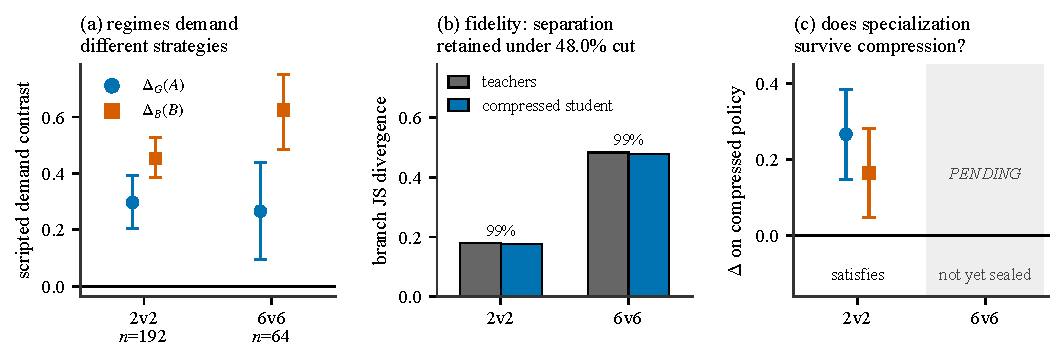
\includegraphics[width=\textwidth]{fig_cross_scale_2v2_6v6.pdf}
\caption{The cross-scale argument in three steps, at $2$v$2$ and $6$v$6$ under one
criterion. (a)~Opponent-regime demand is certified at both scales and does not
weaken with team size---the Regime-$B$ contrast is larger at $6$v$6$.
(b)~Matched-state distillation into a single shared-encoder controller retains
$\approx99\%$ of the teachers' branch divergence at both scales, under a
numerically identical $48.0\%$ reduction in unique actor parameters.
(c)~Whether that compressed policy still satisfies the specialization criterion:
sealed and satisfied at $2$v$2$; the $6$v$6$ cell is drawn as pending because its
evaluation is not yet sealed, and is never estimated.
Error bars are $95\%$ bootstrap CIs.}
\label{fig:crossscale}
\end{figure*}

%----------------------------------------------------------------------
\subsection{The opponent regimes demand different strategies at both scales}
\label{sec:results-demand}

Before asking whether a controller \emph{discovers} two strategies, we establish
that the environment \emph{requires} them. A preregistered opponent-conditioned
protocol scores scripted guard-style and breach-style team responses against each
regime on paired seeds, and certifies demand only if each response strictly beats
the other on its own regime with $\mathrm{LCB}_{95}>0$.

At $2$v$2$ ($n{=}192$ paired seeds), the payoff gaps are
\[
\Delta_G(A)=+0.297\;[+0.203,+0.391],
\qquad
\Delta_B(B)=+0.453\;[+0.385,+0.526],
\]
with concealment gates satisfied on both regimes ($p_C(A)=0.943$,
$p_C(B)=0.917$), so the regime is not identifiable from a single observation.

At $6$v$6$ ($n{=}64$ paired seeds), the poles are size-normalized---the defensive
trigger scales with team size, and the guard response distributes
$\lceil N/2 \rceil$ defenders rather than stacking them on one intruder---and the
same protocol certifies demand with
\[
\Delta_G(A)=+0.266\;[+0.094,+0.438],
\qquad
\Delta_B(B)=+0.625\;[+0.484,+0.750].
\]
Two features matter for the scaling argument (Fig.~\ref{fig:crossscale}a). First,
demand does not weaken with team size: the Regime-$B$ contrast is substantially
\emph{larger} at $6$v$6$ ($+0.625$ vs.\ $+0.453$), driven by guard-style play
collapsing against the breach regime ($0.078$ win rate) while breach-style play
holds ($0.703$). Second, both regimes remain contested rather than saturated at
both scales, so the downstream specialization contrasts are informative.

Certified demand is a property of the environment. It does not predict that a
learned controller will discover the two strategies, and the remainder of this
section is about that gap.

%----------------------------------------------------------------------
\subsection{Independent experts realize the demand as complementary payoff}
\label{sec:results-experts}

Independent PPO experts $\pi_A,\pi_B$ trained against the two regimes satisfy the
specialization criterion at $2$v$2$ on a held-out $64$-seed block:
\[
\Delta_A = +0.172\;[+0.016,+0.328],
\qquad
\Delta_B = +0.297\;[+0.125,+0.469],
\]
while a mixed-opponent generalist trained on the same budget attains
$V(\pi_G,A)=0.375\;[0.265,0.500]$ and $V(\pi_G,B)=0.500\;[0.375,0.625]$---it
does not recover either specialist's own-regime advantage
(Fig.~\ref{fig:winrate-context}).

To separate ``the strategies exist'' from ``the evaluation path can express
them,'' we score a Share-0 reference: bit-exact $z$ dispatch between the verbatim
experts, with zero tied modules. On the matched $128$-seed block it satisfies the
criterion with
\[
\Delta_A = +0.289\;[+0.164,+0.406],
\qquad
\Delta_B = +0.258\;[+0.141,+0.375],
\]
establishing the ceiling that any shared policy is measured against.

At $6$v$6$, specialists are trained under the identical recipe, budget, and
checkpoint rule and serve as distillation teachers. We deliberately do not
re-certify expert crossover or rebuild the Share-0 ladder at $6$v$6$: the
mechanism and its breaking point were localized at $2$v$2$, and the $6$v$6$ track
is a scaling test of the rung that survived, not a rediscovery of the ladder.
This is the one structural asymmetry between the scales, and it is a scope
decision rather than a missing measurement.

%----------------------------------------------------------------------
\subsection{Distillation fidelity licenses the payoff question---it does not
answer it}
\label{sec:results-fidelity}

Matched-state distillation transfers the two experts into discrete modes $z_0,z_1$
of a single controller whose perception encoder is tied ($96.0\%$ of one branch's
parameters) and whose remaining capacity stays private per mode.

Imitation fidelity is high at both scales. At $2$v$2$, holdout argmax agreement
with the source experts is $0.967/0.989$, and the student's branch
Jensen--Shannon divergence is $0.178$ against the experts' own $0.179$. At
$6$v$6$, holdout agreement is $0.963/0.961$ with holdout
$\mathrm{KL}=0.054/0.094$, and the student reproduces $0.478$ of the teachers'
$0.484$ branch divergence. In both cases the student retains roughly $99\%$ of the
behavioral separation present in its teachers (Fig.~\ref{fig:crossscale}b), and a
save/load round trip reproduces logits exactly. Note that the $6$v$6$ teachers are
far more behaviorally distinct in absolute terms ($0.484$ vs.\ $0.179$), so the
compressed policy is asked to preserve a substantially wider separation at the
larger scale.

These are necessary conditions, not the claim. The $2$v$2$ ladder supplies the
counterexample that forces this distinction: Share-Macro retains $0.936/0.969$
agreement---high by any imitation standard---and still \emph{fails} the
specialization criterion (Fig.~\ref{fig:hierarchy}). Action-level agreement and
nonzero action-distribution separation can both survive while closed-loop payoff
specialization does not. Fidelity is therefore reported as a precondition for
asking the payoff question at each scale, and the criterion is what answers it.

\begin{figure}[t]
\centering

\includegraphics[width=\columnwidth]{fig_2v2_measurement_hierarchy.pdf}
\caption{Measurement hierarchy: high imitation and nonzero action-distribution
separation do not imply closed-loop payoff specialization. Share-Macro retains
strong expert agreement yet fails the criterion via
$\mathrm{LCB}_{95}(\Delta_A)=0$.}
\label{fig:hierarchy}
\end{figure}

%----------------------------------------------------------------------
\subsection{Sharing only perception preserves specialization; sharing more
erodes it}
\label{sec:results-ladder}

At $2$v$2$ we sweep how much of the controller is tied, holding the distillation
recipe fixed, and score each rung on the same $128$ seeds
(Table~\ref{tab:sharing-results}, Fig.~\ref{fig:sharing-ladder}).

Sharing only the perception encoder preserves the criterion on both regimes with
no detectable paired loss against Share-0 ($D_A=-0.023$, $D_B=-0.094$; both
$\mathrm{UCB}_{95}\ge0$), while removing $48.0\%$ of the unique actor parameters.
Tying the backbone still satisfies the absolute criterion but now shows a
detectable Regime-$A$ loss, with on-regime performance falling and cross-regime
performance rising---the signature of homogenization rather than uniform
capacity loss. Tying the macro layer fails the criterion outright
($\mathrm{LCB}_{95}(\Delta_A)=0$) and additionally falls outside the imitation
fidelity band, so its degradation is reported as sharing-associated and
fit-confounded rather than uniquely attributed to homogenization.

The engineering consequence is sharp: essentially all of the parameter saving is
already captured by sharing perception alone. Backbone and macro sharing add only
about $1.5$ percentage points of further reduction while progressively destroying
the property the compression was meant to retain.

\begin{table}[t]
\centering
\caption{Parameter--specialization tradeoff on the matched $128$-seed set
($2$v$2$). Unique actor parameters are sealed construction counts. Reduction is
relative to Share-0. $D_A$/$D_B$ are within-seed differences vs.\ Share-0;
``detectable loss'' means $\mathrm{UCB}_{95}(D)<0$.}
\label{tab:sharing-results}
\begin{tabular}{@{}lrrlll@{}}
\toprule
\textbf{Condition} & \textbf{Params (M)} & \textbf{Red.} &
$\boldsymbol{\Delta_A}$ & $\boldsymbol{\Delta_B}$ &
\textbf{Criterion / $D$} \\
\midrule
Share-0
  & $6.947$ & $0\%$
  & $+0.289\;[+0.164,+0.406]$
  & $+0.258\;[+0.141,+0.375]$
  & PASS (reference) \\
Share-Encoder
  & $3.613$ & $\mathbf{48.0\%}$
  & $+0.266\;[+0.148,+0.383]$
  & $+0.164\;[+0.047,+0.281]$
  & PASS; no detectable loss \\
Share-Backbone
  & $3.509$ & $49.5\%$
  & $+0.148\;[+0.023,+0.266]$
  & $+0.141\;[+0.016,+0.266]$
  & PASS; detectable loss on $A$ \\
Share-Macro
  & $3.508$ & $49.5\%$
  & $+0.125\;[0.000,+0.250]$
  & $+0.156\;[+0.031,+0.281]$
  & FAIL ($\mathrm{LCB}_{95}(\Delta_A)=0$) \\
\bottomrule
\end{tabular}
\end{table}

\begin{figure*}[t]
\centering

\includegraphics[width=\textwidth]{fig_claim_a_2v2.pdf}
\caption{Causal chain at $2$v$2$.
(a)~Independent PPO experts establish complementary payoff strategies.
(b)~Matched-state distillation transfers them into discrete modes of one
shared-encoder controller ($z_0\!\sim\!\pi_A$, $z_1\!\sim\!\pi_B$).
(c)~Sealed $\Delta_A,\Delta_B$ with $95\%$ CIs across progressive sharing
($n{=}128$). Share-0 is a bit-exact expert-dispatch control; the remaining rungs
share one distillation recipe and differ only in which modules are tied.}
\label{fig:claim-a}
\end{figure*}

\begin{figure*}[t]
\centering
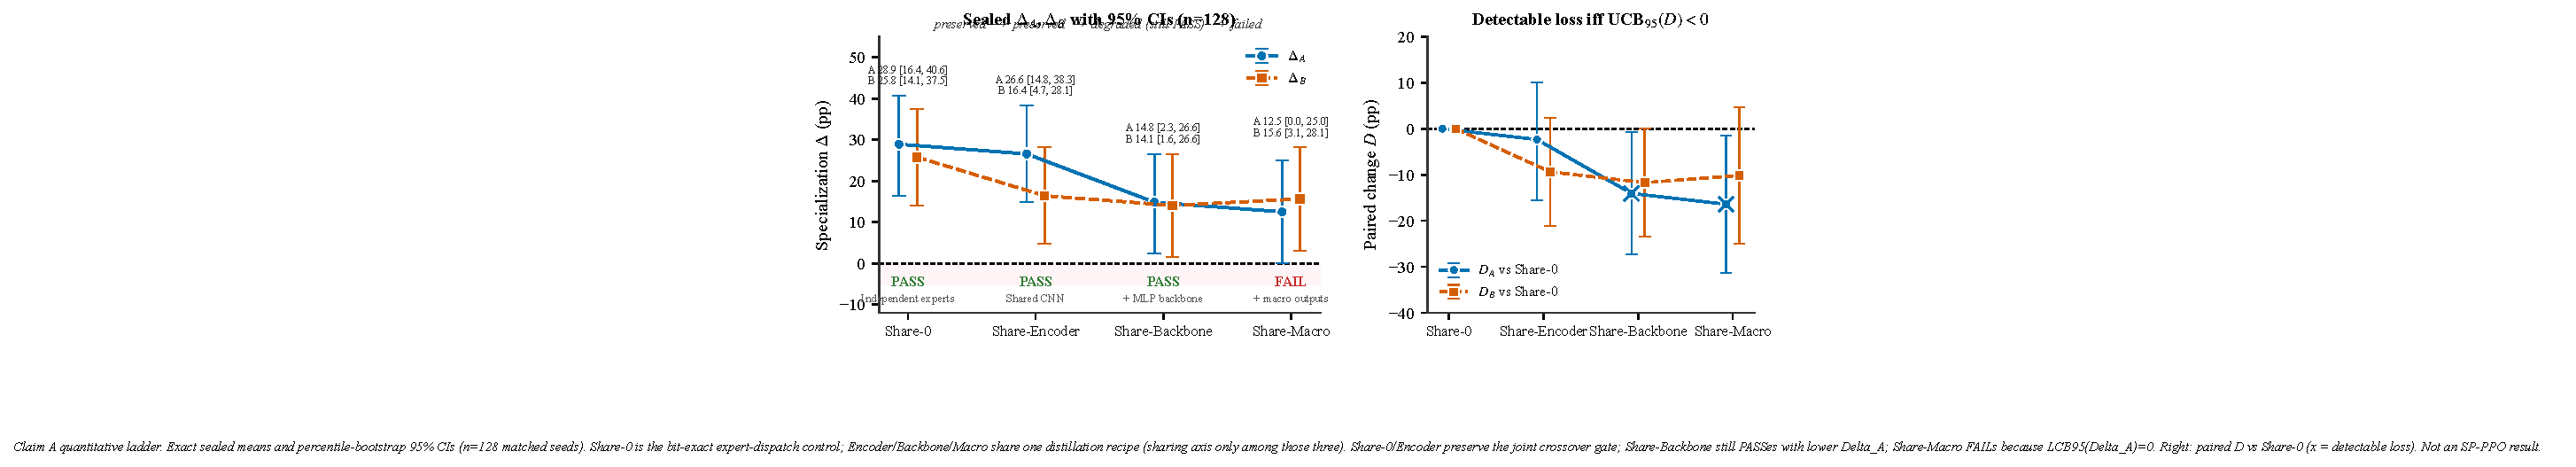
\includegraphics[width=\textwidth]{fig_sharing_ladder_2v2.pdf}
\caption{Exact sealed $\Delta_A,\Delta_B$ (left) and paired $D$ vs.\ Share-0
(right) with $95\%$ CIs ($n{=}128$). Share-Backbone still satisfies the absolute
criterion but already shows detectable Pole-$A$ loss; Share-Macro fails because
$\mathrm{LCB}_{95}(\Delta_A)=0$.}
\label{fig:sharing-ladder}
\end{figure*}

\begin{figure*}[t]
\centering

\includegraphics[width=\textwidth]{fig_absolute_winrate_context_2v2.pdf}
\caption{Absolute win rates for the mixed-opponent generalist $\pi_G$, the
independent experts, and the shared-encoder modes against both regimes. The
crossover pattern is visible when A-specialized policies win more on Regime~$A$
and B-specialized policies win more on Regime~$B$. Absolute context only;
specialization is decided by the paired $\Delta$ criterion. Error bars are $95\%$
bootstrap CIs ($\pi_G$/experts $n{=}64$; shared encoder $n{=}128$).}
\label{fig:winrate-context}
\end{figure*}

%----------------------------------------------------------------------
\subsection{Does the preserved rung survive scale?}
\label{sec:results-scale}

The $2$v$2$ ladder identifies exactly one configuration worth carrying forward:
shared perception, private strategy capacity. At $6$v$6$ we rebuild that single
configuration---same architecture, same distillation recipe, same $48.0\%$
parameter reduction---and evaluate it against the same criterion on a fresh
$128$-seed block, with $z_0$ and $z_1$ dispatched from one checkpoint
(Fig.~\ref{fig:crossscale}c).

% ---------------------------------------------------------------- PENDING-6V6
% The sealed 6v6 crossover evaluation is the only number in this section that is
% not yet available. Evaluation launched 2026-09-11T18:33Z on seeds
% 13640001..13640128 (512 episodes, ~62 s/ep). On completion, replace the
% placeholder below with the sealed values from
%   artifacts/strategic_demand/sppo/RUNG1_6V6_CROSSOVER_EVAL_RESULT.json
%     -> PRIMARY_GATE.delta_A {mean, lcb95, ucb95}
%     -> PRIMARY_GATE.delta_B {mean, lcb95, ucb95}
%     -> PRIMARY_GATE.passes
% If RUNG1_6V6_CROSSOVER_EVAL_INTEGRITY_REQUIRED.json is written instead, a tie or
% reversal was flagged and a row-level audit is required BEFORE any sentence here
% is written.
% ----------------------------------------------------------------------------
\noindent
\textbf{[PENDING-6V6 --- sealed crossover in progress; do not typeset.]}
\[
\Delta_A = \texttt{<pending>},
\qquad
\Delta_B = \texttt{<pending>}.
\]

\noindent
The interpretation is pre-committed and does not depend on the outcome. If the
criterion is satisfied, the same shared-perception compression that preserved
complementary specialization with two agents also preserves it with six, and the
$48\%$ deployment saving transfers to a materially harder coordination problem.
If it is not satisfied, the compression result is scale-bounded: the location of
the sharing boundary established at $2$v$2$ does not by itself license deployment
at larger team sizes, and the boundary must be re-established per scale. Either
outcome is reported against the same criterion, and no rung beyond shared
perception is evaluated at $6$v$6$ in this work.

%----------------------------------------------------------------------
\subsection{What the latent modes actually do}
\label{sec:results-behavior}

Three complementary views establish that the modes correspond to recognizable
team strategies rather than to arbitrary policy perturbations: matched
trajectories, role-allocation proxies, and the payoff contrasts already reported.

Under identical initial conditions with only $z$ changed, the team paths diverge
at tick~$4$ and reach different terminal outcomes, with terminal scores matched
against the sealed evaluation rows (Fig.~\ref{fig:traj}); matched frames at a
fixed tick show the same seed under both codes and both regimes
(Fig.~\ref{fig:qual}). Role-allocation telemetry
(Figs.~\ref{fig:roles}--\ref{fig:roles-ext}) is reported as an exploratory
characterization at $n{=}24$ per cell: coarse means are largely regime-driven,
with smaller within-regime gaps between codes. We therefore treat role proxies as
descriptive support for the trajectory evidence, never as a specialization gate.

\begin{figure*}[t]
\centering

\includegraphics[width=0.92\textwidth]{fig_trajectory_strip_2v2.pdf}
\caption{Matched seed $11960003$, shared-encoder policy: identical initial
conditions within each panel; only forced $z$ differs. Solid~$z_0$, dashed~$z_1$;
stars mark first action divergence ($t{=}4$). Terminal scores match the sealed
evaluation rows. Visual evidence that changing $z$ changes team behavior---not a
substitute for the statistical criterion.}
\label{fig:traj}
\end{figure*}

\begin{figure*}[t]
\centering

\includegraphics[width=0.95\textwidth]{fig_qualitative_latent_2v2.pdf}
\caption{Matched-frame grid at tick~$30$ for the same seed and shared-encoder
policy. Columns differ only in forced $z$; rows differ only in opponent regime.}
\label{fig:qual}
\end{figure*}

\begin{figure*}[t]
\centering

\includegraphics[width=\textwidth]{fig_role_allocation_2v2.pdf}
\caption{Role-allocation proxies under forced $z_0$ vs.\ $z_1$ on both regimes
(defender count, attacker count, attack/defense ratio). Episode-mean telemetry
from an exploratory characterization ($n{=}24$/cell; not a specialization gate).}
\label{fig:roles}
\end{figure*}

\begin{figure*}[t]
\centering

\includegraphics[width=\textwidth]{fig_latent_behavior_2v2.pdf}
\caption{Extended role telemetry (same exploratory source as
Fig.~\ref{fig:roles}): defenders, attackers, intercept near enemy carrier, carrier
escort, and attack/defense ratio under forced $z_0$ vs.\ $z_1$ ($n{=}24$/cell).
Regime effects dominate; within-regime gaps between codes remain modest.}
\label{fig:roles-ext}
\end{figure*}

%----------------------------------------------------------------------
\subsection{Robustness as a sim-to-real diagnostic}
\label{sec:results-robustness}

Specialization that exists only under noiseless sensing is not a deployable
property. We therefore re-evaluate the preserved $2$v$2$ configuration under three
deployment-relevant perturbation families at a preregistered severity ladder,
scoring the same criterion at each dose on the same $128$ seeds
(Fig.~\ref{fig:robust}). Severities were fixed in the protocol before any
robustness episode ran, and no severity was added after seeing a result.

The three families dissociate cleanly. Localization noise leaves the criterion
satisfied at every tested dose, with paired changes relative to nominal
statistically indistinguishable from zero---specialization is genuinely robust to
this channel across the tested range. Motion error fails the joint criterion at
\emph{every} nonzero dose, always through Regime~$B$, and---critically---the
failure does not grow with severity: the mildest dose already reproduces it, and
no paired degradation interval excludes zero. The honest description is a
persistently fragile Regime-$B$ margin under any motion perturbation, not a
dose-dependent breakdown. Control latency behaves differently again: it is the one
family with a monotone dose response, concentrated entirely in Regime~$A$, whose
margin falls steadily as latency increases and reaches the boundary of statistical
detectability at the largest authorized dose.

That the three families fail in three different ways---not at all, immediately and
flatly, and monotonically---is itself the finding. It means ``robustness'' is not
a single scalar property of the compressed controller, and that a deployment
decision must be made per sensing channel rather than from an aggregate score.

\begin{figure*}[t]
\centering

\includegraphics[width=\textwidth]{fig_robustness_delta_dose.pdf}
\caption{Dose--response of specialization under deployment-relevant perturbations
($n{=}128$): localization (GPS-like), motion (currents/actuators), and control
latency (communications). \textsc{pass}/\textsc{fail} mark the specialization
criterion at each severity. Localization remains specialized at every tested dose;
motion breaks Regime-$B$ specialization from the first nonzero dose; latency shows
monotone Regime-$A$ erosion.}
\label{fig:robust}
\end{figure*}

%----------------------------------------------------------------------
\subsection{Scope}
\label{sec:results-scope}

Three limits bound these claims. First, the sharing ladder is localized at $2$v$2$
only; $6$v$6$ evaluates the single preserved rung, so the \emph{position} of the
sharing boundary is established at one scale and tested, not re-derived, at the
other. Second, robustness is characterized at $2$v$2$ across three families and a
preregistered severity ladder; the corresponding $6$v$6$ seed block is reserved
but not yet spent, so no cross-scale robustness claim is made. Third,
strategy-preserving fine-tuning interventions (formulated in the supplementary
material) did not recover the criterion under frozen matched protocols, and are
not credited for any result above.

\section{Discussion}
\label{sec:discussion}
%======================================================================

The primary scientific finding concerns progressive parameter sharing:
perception-level sharing (Share-Encoder) preserves the specialization criterion
under the matched-seed protocol, with a decomposition consistent with mild
strategy homogenization rather than on-regime specialization loss. Deeper
sharing of the MLP backbone (Share-Backbone) remains fidelity-comparable and
still clears the absolute specialization criterion, yet produces a detectable
paired reduction relative to Share-0 on Regime~A, consistent with specialization
loss under additional representation sharing. Further sharing at macro-action
outputs (Share-Macro) coincides with deteriorated imitation fidelity and failure
of the specialization criterion; under the imitation-fidelity control, that
degradation is reported as sharing-associated but not uniquely attributed to a
single interference mechanism.

The centerpiece is architectural and experimental, not algorithmic PPO novelty:
independently learned strategies are encoded as discrete modes of shared
controllers under a common distillation recipe, validated by closed-loop
crossover at Share-Encoder, and then subjected to controlled progressive
sharing. Share-0 is the bit-exact expert-dispatch reference; Enc$\rightarrow$Back$\rightarrow$Macro
is the clean sharing axis. Attempted PPO interventions (CSC/SPFT) remain a
sealed non-recovery side study in the supplementary material and are not the
method that produced Share-Encoder PASS.

For multi-robot policy design, the sharing study suggests that substantial
perception sharing can be tolerable in this setting, while sharing deeper
decision-related representations is where opponent-conditioned specialization
becomes fragile. Claims remain scoped to the two-regime nominal $2$-vs-$2$ task
and training recipes studied here. External validity for larger teams and
sensing/control perturbations remains outside the primary claim until those
experiments are finished.

%======================================================================

\section{Conclusion}
\label{sec:conclusion}
%======================================================================

We use standard opponent-specific PPO to learn complementary multi-robot
experts, distill their matched-state behaviors into discrete modes of shared
strategy-conditioned controllers under a common recipe, and progressively tie
policy modules to identify where closed-loop specialization survives or
collapses. Share-Encoder preserves specialization; Share-Backbone introduces a
detectable paired loss on one regime despite comparable fidelity; Share-Macro
yields fit-confounded degradation with failure of the specialization criterion.
High imitation alone does not guarantee payoff-level specialization. Claims
remain scoped to the nominal $2$-vs-$2$, two-regime setting and training recipes
studied here.


% Optional appendix for CSC/SPFT sealed non-recovery (page budget)
% \appendix
% \input{sections/99_appendix_spp}

\bibliographystyle{IEEEtran}
% \bibliography{refs}  % enable once refs.bib is populated

\end{document}
